\documentclass[a4paper,10pt]{article}

%\usepackage{times}
\usepackage{geometry}
\usepackage{amsmath}
\usepackage{amssymb}
\usepackage{mathtools}
\usepackage{graphicx}
\usepackage{float}
\usepackage{color}
\usepackage{booktabs, makecell}
\usepackage{psfrag}
\usepackage{hyperref}
\usepackage{enumitem}
\usepackage{tablefootnote}
\usepackage{eurosym}
\usepackage[UKenglish]{isodate}
\usepackage{listings}
%\usepackage{auto-pst-pdf}
\geometry{a4paper,margin=25mm,heightrounded}

\newif\ifsolution
\solutiontrue

\newcounter{exercisecounter}
\newcounter{problemcounter}
\newcounter{taskcounter}
\newenvironment{problem} [1][]
{\noindent\ignorespaces\stepcounter{problemcounter}\large \textbf{Problem \arabic{exercisecounter}: #1}\normalsize\vspace{0.1cm}\\}
{\par\noindent\ignorespacesafterend\vspace{0.1cm}}
\newcommand{\task}[1]{\vspace{0.0cm}\par\noindent\stepcounter{taskcounter}\textbf{Problem \arabic{exercisecounter}.\arabic{taskcounter}}: #1}
\newcommand{\sol}[0]{\vspace{0.2cm}\par\noindent\stepcounter{taskcounter}\textbf{\arabic{exercisecounter}.\arabic{problemcounter}.\arabic{taskcounter}}: }
\newcommand{\inlinesol}[1]{\vspace{0.2cm}\par\noindent\textit{#1}\vspace{0.2cm}}


\let\olddescription\description
\renewcommand{\description}{
  \olddescription
  \setlength{\itemsep}{1pt}
  \setlength{\parskip}{1pt}
  \setlength{\parsep}{0pt}
}

\let\olditemize\itemize
\renewcommand{\itemize}{
  \olditemize
  \setlength{\itemsep}{3pt}
  \setlength{\itemindent}{0pt}
  \setlength{\parskip}{1pt}
  \setlength{\parsep}{0pt}
}

\let\oldenumerate\enumerate
\renewcommand{\enumerate}{
  \oldenumerate
  \setlength{\itemsep}{3pt}
  \setlength{\itemindent}{0pt}
  \setlength{\parskip}{1pt}
  \setlength{\parsep}{0pt}
}

\newcommand{\comm}[1]{}

\setlength{\parindent}{0pt}
\setlength{\parskip}{6pt}

\ifsolution
\newcommand{\solution}[1]{\par\noindent\textit{Solution: #1}}
\else
\newcommand{\solution}[1][]{}
\fi


\setcounter{exercisecounter}{2}
\setcounter{problemcounter}{1}
\begin{document}
\Large\noindent\textsc{Fundamentals of Artificial Intelligence}\\
\large\noindent Programming Exercise \arabic{exercisecounter}: Constraint Satisfaction Problem \hfill 18 November 2022\\
Yuanfei Lin, \hfill {\small(last updated \today)}\\
Deyu Fu, Sebastian Mair, Yingjie Xu, Ziyue Zhang (in alphabetical order by last name)\\ \vspace{0.8cm}

\begin{problem}[Organizing Water Sports]

\noindent \textbf{Task Desription}

You are the organizer of a water sports club, which provides 4 activities: \textbf{Stand-Up Paddle}, \textbf{Windsurf}, \textbf{Catamaran} and \textbf{Kayak}. Today, a group of 8 students arrived, namely \textbf{Anna, Barney, Claire, Davin, Elena, Freddy, Gloria, and Henry}. They haven't decided which one to participate in and ask for your help.

\begin{figure}[H]
	\begin{center}
		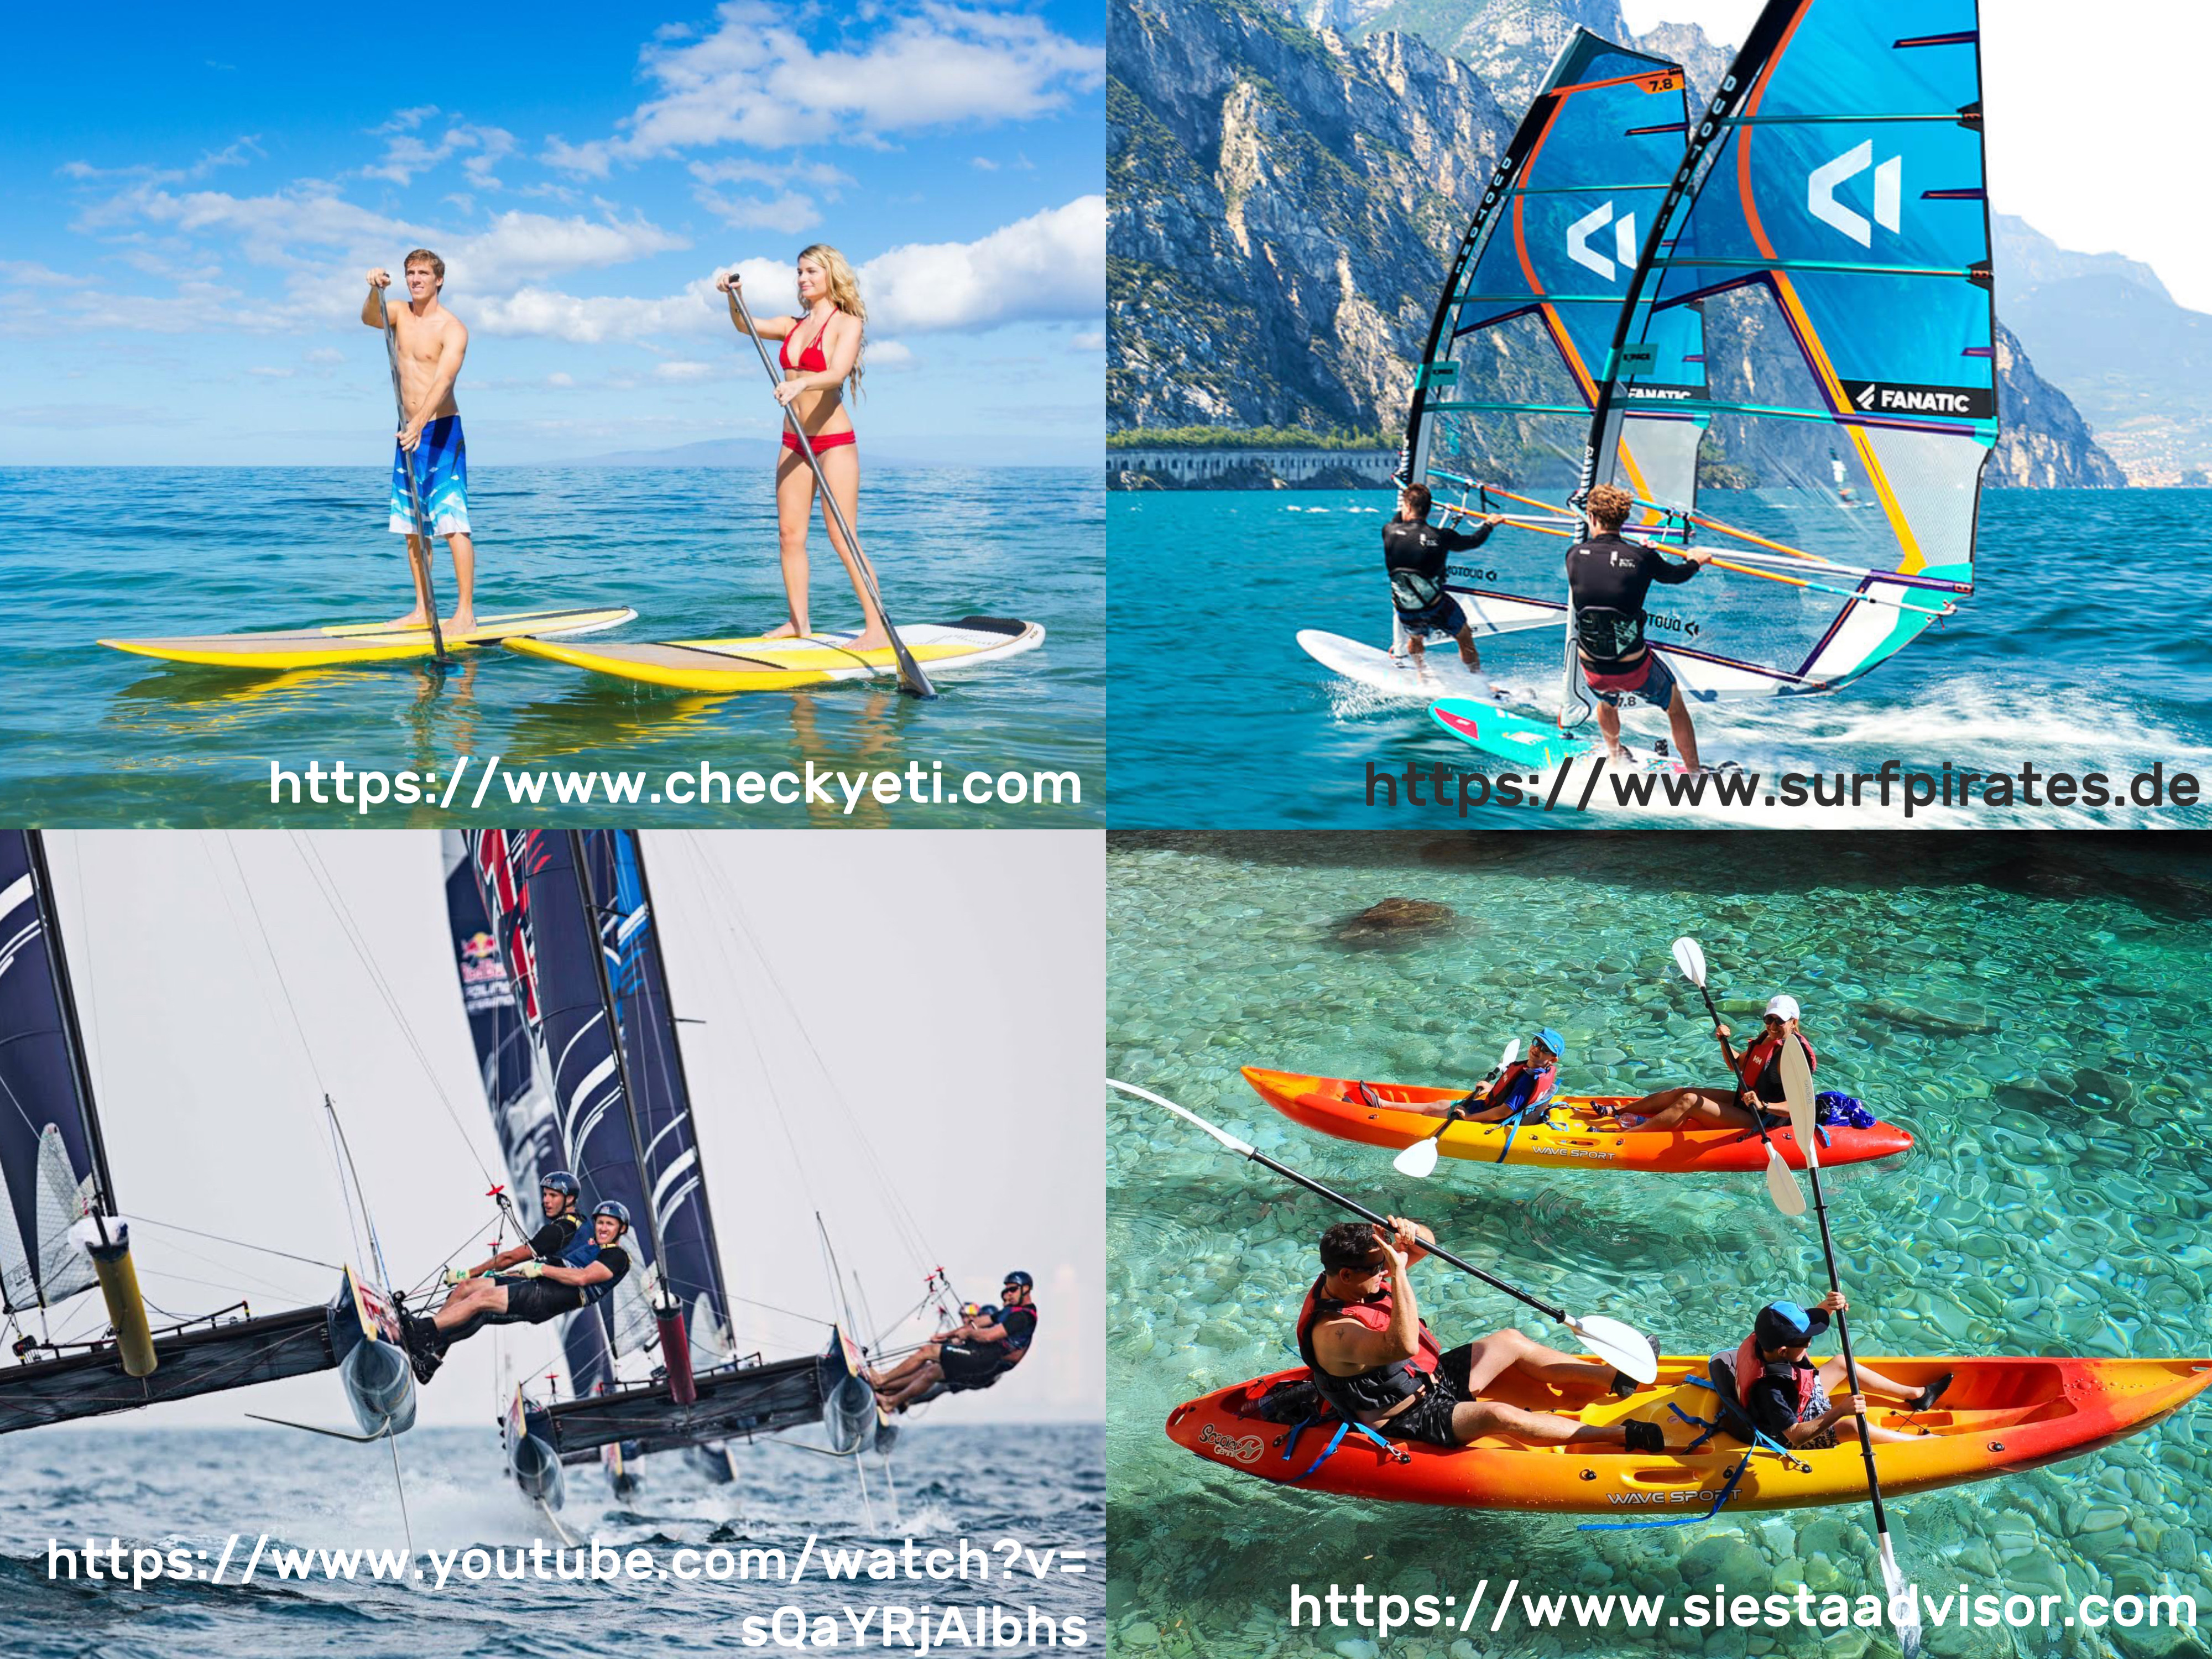
\includegraphics[width=0.9\linewidth]{./sports.jpg}
	\end{center}

	\caption{Different kinds of water sports.}

	\label{water sports}
\end{figure}

The information about the provided activities is listed below:

\begin{table}[h]
	\begin{center}
		\begin{tabular}{c|c|c}
			\toprule
			\textbf{Activity}        & \textbf{Person per boat/board} & \textbf{Price per boat/board}\tablefootnote{Note that the price includes the cost of the whole equipment set.} \\
			\hline
			Stand-Up Paddle & 1               & 6 \euro{}      \\
			\hline
			Windsurf        & 1               & 10 \euro{}     \\
			\hline
			Catamaran       & 2               & 15 \euro{}     \\
			\hline
			Kayak           & 2               & 10 \euro{}     \\
			\bottomrule
		\end{tabular}
	\end{center}
	\label{known}
\end{table}
\newpage
Note that:
\begin{itemize}

	\item These are merely 4 programs planned, which don't necessarily have to all take place. Which program(s) is/are actually going to take place depend(s) on the given constraints.
	\item Odd-numbered participants can also take part in Catamaran and Kayak, which means they will share the boat with strangers and pay half of the price.
	\item Every student can take part in \textbf{at most} 1 program. Students would be assigned to the program they want to attend by default if there are no additional statements.
\end{itemize}

%Note that these are merely 4 topics planned, which don't necessarily have to take place all. Which topic(s) is/are actually going to be presented depend(s) on the given constraints.
Now consider the following constraints:

\vspace{-0.1cm}
\begin{enumerate}


	\item Elena and Freddy are good friends. They want to participate in a program where they can share a boat.
	\item None of them want to share a boat with strangers.
	\item Stand-up paddle is popular today, so there are only 3 spaces left.
	\item Barney doesn’t know how to swim, so he doesn’t want to be in a program alone, otherwise he won't attend any program.
	\item Elena and Gloria are good friends, such that they want to attend the same program or not attend any program.
	\item Davin has a great passion for kayaking, so he either chooses kayak or nothing.
	\item If Henry participates in a program, he is okay with any of them, except stand-up paddle.
	\item Freddy neither wants to be in the same program as Henry nor stay on the shore together with him.
	\item Anna wants to go either windsurfing or catamaran sailing. Otherwise, she will not attend any program.
	\item Barney chooses to sail catamarans, and Claire is willing to teach him and join the same program.
	\item The group has a limited budget so the total cost cannot exceed 60 \euro{}.
	\item Anna, Davin, and Henry want to be together in the same activity, otherwise they are all willing to  wait on shore.
	\item Davin chooses to play SUP with his dog, but Elena is afraid of dogs, so she cannot join him.
	\item No one wants to participate in an activity alone from the group. Otherwise, they don't participate in any activities.
	\item If the group wants to attend windsurfing, they need to join a course with an instructor, which requires at least 3 participants to start.
	\item The group wants to experience as much as possible, they wish to participate in at least 3 programs.


\end{enumerate}


Model the constraint satisfaction problem in \textsc{Python}. For each of the following subsets of constraints, find the solution, if it exists:


\task{\{ 1 - 7, 9 - 11, 14, 15 \}}

\task{\{ 7 - 16 \}}

\task{\{ 1 - 3, 5, 7, 11, 12, 16 \}}

\task{\{ 1, 4, 5, 11 - 16 \}}

\task{\{ 2 - 12, 15 \}}

\task{\{ 1 - 11, 14  \}}

Note that not all problems can be satisfied.

\newpage
\end{problem}

\noindent \textbf{Programming Framework}

\normalsize
For this programming exercise, a \textit{Jupyter Notebook} will be used. To model the constraint satisfaction problem, you should know or look up Python's lambdas, lists and dictionaries. The main function of the template is in the \textbf{csp.ipynb} file, which is also the only file you have to work on. An example, on how to model a constraint satisfaction problem using the \textit{AIMA}, is provided in the notebook \textbf{csp\_demo.ipynb}. This example is taken from Exercise 3.4. 
The following steps are required to correctly set up the environment for the programming exercise and submission:

\begin{enumerate}
	\item \textbf{Installation of AIMA}: Work through AIMA installation instructions on Moodle\footnote{\href{https://www.moodle.tum.de/mod/page/view.php?id=2323882}{https://www.moodle.tum.de/mod/page/view.php?id=2323882}} (Using Docker is recommended for beginners)
	\item \textbf{ARTEMIS}: Log into ARTEMIS\footnote{\href{https://artemis.ase.in.tum.de/courses/222/exercises}{https://artemis.ase.in.tum.de/courses/222/exercises}} with your TUM credentials. Find the exercise \textit{Constraint Satisfaction Problems} and follow the installation and submission instructions.
\end{enumerate}

%
%For this programming exercise, a \textit{Jupyter Notebook} will be used. The template for the exercise can be found in ARTEMIS\footnote{\href{https://artemis.ase.in.tum.de/courses/159/exercises}{https://artemis.ase.in.tum.de/courses/159/exercises}}. To model the constraint satisfaction problem, you should know or look up Python's lambdas, lists and dictionaries. The following steps are required to correctly set up the environment for the programming exercise:
%
%\begin{enumerate}
%	\item \textbf{Installation of Environment and Download of the AIMA python code} If you do not already have the \textit{Jupyter Notebook} environment installed on your machine, the installation is the first step you have to perform. We recommend installing via \textit{Docker} since this will set up the whole environment for you. The template for the programming exercise is based on the code from the \textit{AIMA python}\footnote{\href{https://github.com/aimacode/aima-python}{https://github.com/aimacode/aima-python}} project. Therefore, if you want to use Anaconda to set up the environment, you first have to download the code from this project before the template can be used. Instructions for installation of Anaconda and AIMA python code can be found in ``AIMA Code Installation Instructions'' on Moodle\footnote{\href{https://www.moodle.tum.de/pluginfile.php/3159598/mod\_resource/content/5/AIMAinstallation.pdf}{https://www.moodle.tum.de/pluginfile.php/3159598/mod\_resource/content/5/AIMAinstallation.pdf}}.
%	\item \textbf{Pull of the template:} Pull the repository with the template from ARTEMIS, which can be done similarly to AIMA python just with the repository link from ARTEMIS. To avoid issues with the relative file paths, we recommend copying all files contained in the template into the root directory of the \textit{AIMAcode} project that you downloaded in the previous step.
%\end{enumerate}
%
%After completing the above steps, you are all set up to start with the exercise. The main function of the template is the \textit{Jupyter Notebook} \textbf{csp.ipynb}, which is also the only file you have to work on. Your task is to model the Organizing Water Sports problem. An example, of how to model a constraint satisfaction problem using the \textit{AIMAcode}, is provided in the notebook \textbf{csp\textunderscore demo.ipynb}. This example is taken from Exercise 3.4.
%
%
%\noindent \large \textbf{Submission}
%
%\normalsize
%For submission, you have to upload the following files in ARTEMIS:
%\vspace{-0.5cm}
%\begin{enumerate}
%	\item Copy \textbf{csp.ipynb} (notebook containing your solution for modeling the Organizing Water Sports problem) to the pulled repository.
%	\item Add and commit the altered notebook and push it to ARTEMIS with
%
%	      \lstset{
%		      %numbers=left,                        % 设置行号
%		      columns=fullflexible,
%		      tabsize=4,                       % 把tab扩展为4个空格,默认是8个太长
%		      %frame=single,                        % 设置有边框
%		      % identifierstyle=\color{red},
%		      language=c++,
%	      }
%
%	      \begin{lstlisting}
%	git add csp.ipynb
%	git commit -m "A commit message"
%	git push
%	\end{lstlisting}
%	      (all within the ARTEMIS repository)
%\end{enumerate}

\textbf{A pass will be awarded only if:}
\vspace{-0.3cm}
\begin{enumerate}
	\item you submitted the \textbf{correct file} with the \textbf{correct name}, as shown above.
	\item you \textbf{did not zip} your file.
	\item you \textbf{pushed your files to your ARTEMIS branch}.
	\item you \textbf{did not change} the \textbf{variable names} provided by us within the template.
	\item your submitted files can be run in a Docker/Anaconda environment (Python 3.7 at least) with the packages provided by the \textit{requirements.txt} in the \textit{aima repository}, the utils.py, the search.py and the csp\_programming\_exercise.py provided by us \textbf{within a reasonable time (under 5 minutes)}.
	\item the problem has been modeled correctly using the NaryCSP class from the module \\ csp\_programming\_exercise.
	\item like the rest of the programming exercises, this is an individual project and you \textbf{must} finish the task on your
	      own. (We will use a plagiarism detection tool and any copied code will annul all bonus exercises
	      from both the copier and the copied person!)
\end{enumerate}


Submission will close on \textcolor{red}{\textbf{Friday, 16.12.2022 at 23:59}}. Your solution will be graded by ARTEMIS. There will be feedback on formatting errors and rightly solved CSP. Nonetheless, it is very important to follow the instructions exactly!

We offer preliminary checks of your solution and ARTEMIS will show your progress. You can submit your solution multiple times and get feedback for each submission. Your final submission will be checked. We award 1 point if all checks including plagiarism pass.



\end{document}